%%%%%%%%%%%%%%%%%%%%%%%%%%%%%%%%%%%%%%%%%%%%%%%%%%%%%%%%%%%%
%%% LIVECOMS ARTICLE TEMPLATE FOR BEST PRACTICES GUIDE
%%% ADAPTED FROM ELIFE ARTICLE TEMPLATE (8/10/2017)
%%%%%%%%%%%%%%%%%%%%%%%%%%%%%%%%%%%%%%%%%%%%%%%%%%%%%%%%%%%%
%%% PREAMBLE
\documentclass[9pt,tutorial,pubversion]{livecoms}
% Use the 'onehalfspacing' option for 1.5 line spacing
% Use the 'doublespacing' option for 2.0 line spacing
% Use the 'lineno' option for adding line numbers.
% Use the "ASAPversion' option following article acceptance to add the DOI and relevant dates to the document footer.
% Use the 'pubversion' option for adding the citation and publication information to the document footer, when the LiveCoMS issue is finalized.
% The 'bestpractices' option for indicates that this is a best practices guide.
% Omit the bestpractices option to remove the marking as a LiveCoMS paper.
% Please note that these options may affect formatting.

\usepackage{lipsum} % Required to insert dummy text
\usepackage[version=4]{mhchem}
\usepackage{siunitx}
\DeclareSIUnit\Molar{M}
\usepackage[italic]{mathastext}
\graphicspath{{figures/}}

%%%%%%%%%% USER INPUT PACKAGES & FUNCTIONS
\usepackage{listings}
\lstset{
	basicstyle=\ttfamily,
	commentstyle={},
	breakatwhitespace=true,
	breaklines=true,
	language=bash
}
\usepackage{pythonhighlight}

%%%%%%%%%%%%%%%%%%%%%%%%%%%%%%%%%%%%%%%%%%%%%%%%%%%%%%%%%%%%
%%% IMPORTANT USER CONFIGURATION
%%%%%%%%%%%%%%%%%%%%%%%%%%%%%%%%%%%%%%%%%%%%%%%%%%%%%%%%%%%%

\newcommand{\versionnumber}{1.0}  % you should update the minor version number in preprints and major version number of submissions.
\newcommand{\githubrepository}{\url{https://github.com/OpenBioSim/biosimspace_tutorials}}  %this should be the main github repository for this article

%%%%%%%%%%%%%%%%%%%%%%%%%%%%%%%%%%%%%%%%%%%%%%%%%%%%%%%%%%%%
%%% ARTICLE SETUP
%%%%%%%%%%%%%%%%%%%%%%%%%%%%%%%%%%%%%%%%%%%%%%%%%%%%%%%%%%%%
\title{A Suite of Tutorials for the BioSimSpace Framework for Interoperable Biomolecular Simulation [Article v\versionnumber]}
% Everyone in alphabetical order other than Lester

\author[1,2*]{Lester O. Hedges}
\author[3\authfn{1}]{Sofia Bariami}
\author[2]{Matthew Burman}
\author[3]{Finlay Clark}
\author[4]{Benjamin P. Cossins}
\author[3]{Adele Hardie}
\author[3]{Anna M. Herz}
\author[3]{Audrius Kalpokas}
\author[5]{Dominykas Lukauskis}
\author[3]{Antonia S.J.S. Mey}
\author[2,3*]{Julien Michel}
\author[3\authfn{2}]{Jenke Scheen}
\author[4]{Miroslav Suruzhon}
\author[1]{Christopher J. Woods}
\author[4]{Zhiyi Wu}

%\author[1,2\authfn{1}\authfn{3}]{Firstname Middlename Familyname}
%\author[2\authfn{1}\authfn{4}]{Firstname Initials Surname}
%\author[2*]{Firstname Surname}
\affil[1]{Advanced Computing Research Centre, University of Bristol, UK}
\affil[2]{OpenBioSim Community Interest Company, UK}
\affil[3]{EaStCHEM School of
Chemistry, University of Edinburgh, UK}
\affil[4]{Exscientia Plc., Oxford, UK}
\affil[5]{Department of Chemistry and Institute of Structural and Molecular Biology, University College London, UK}


\corr{julien.michel@ed.ac.uk}{JM}  % Correspondence emails.  FMS and FS are the appropriate authors initials.
\corr{lester@openbiosim.org}{LH}

\orcid{Lester Hedges}{0000-0002-5624-0500}
\orcid{Matthew Burman}{0000-0001-5360-0024}
\orcid{Sofia Bariami}{0000-0002-5240-7684}
\orcid{Finlay Clark}{0000-0003-0474-5475}
\orcid{Benjamin P. Cossins}{0000-0002-6699-8833}
\orcid{Adele Hardie}{0009-0002-9943-9920}
\orcid{Anna M. Herz}{0000-0003-2831-6691}
\orcid{Audrius Kalpokas}{0000-0002-4579-070X}
\orcid{Dominykas Lukauskis}{0000-0002-4999-2691}
\orcid{Antonia Mey}{0000-0001-7512-5252}
\orcid{Julien Michel}{0000-0003-0360-1760}
\orcid{Jenke Scheen}{0000-0001-9781-0445}
\orcid{Miroslav Suruzhon}{0000-0002-6794-1679}
\orcid{Christopher J Woods}{0000-0001-6563-9903}
\orcid{Zhiyi Wu}{0000-0002-7615-7851}


%\contrib[\authfn{1}]{These authors contributed equally to this work}
%\contrib[\authfn{2}]{These authors also contributed equally to this work}

\presentadd[\authfn{1}]{Cresset Litlington SG8 0SS, Cambridgeshire,
UK}
\presentadd[\authfn{2}]{Open Molecular Science Foundation, 200 B Street, Suite F, Davis CA 95616, USA}
%\presentadd[\authfn{4}]{Department, Institute, Country}

\blurb{This LiveCoMS document is maintained online on GitHub at \githubrepository; to provide feedback, suggestions, or help improve it, please visit the GitHub repository and participate via the issue tracker.}

%%%%%%%%%%%%%%%%%%%%%%%%%%%%%%%%%%%%%%%%%%%%%%%%%%%%%%%%%%%%
%%% PUBLICATION INFORMATION
%%% Fill out these parameters when available
%%% These are used when the "pubversion" option is invoked
%%%%%%%%%%%%%%%%%%%%%%%%%%%%%%%%%%%%%%%%%%%%%%%%%%%%%%%%%%%%
\pubDOI{10.33011/livecoms.5.1.2375}
\pubvolume{5}
\pubissue{1}
\pubyear{2023}
\articlenum{2375}
\datereceived{20 July 2023}
\dateaccepted{13 December 2023}

%%%%%%%%%%%%%%%%%%%%%%%%%%%%%%%%%%%%%%%%%%%%%%%%%%%%%%%%%%%%
%%% ARTICLE START
%%%%%%%%%%%%%%%%%%%%%%%%%%%%%%%%%%%%%%%%%%%%%%%%%%%%%%%%%%%%

\begin{document}

\begin{frontmatter}
\maketitle

\begin{abstract}
This tutorial serves as a getting-started guide for BioSimSpace (BSS), an interoperable molecular simulation framework, that allows simulations with different sets of molecular dynamics software packages. This tutorial will cover four main use cases for BioSimSpace. The introductory tutorial introduces the basic structure of BioSimSpace, how to use the API to access functionality, and how to write code for setting up and running standard molecular dynamics simulations. Three advanced use cases of BSS are then provided, describing how to set up and run a funnel metadynamics simulation, steered molecular dynamics, and relative or absolute alchemical binding free energy calculations. 
\end{abstract}

\end{frontmatter}


\section{Introduction}

BioSimSpace (BSS)~\cite{bss_paper} 
 (\url{http://openbiosim.biosimspace.org}) is a software that allows the setup, simulation, and analysis of different types of molecular dynamics (MD) simulation methodologies with different software packages. The software provides a common API in Python for the following MD software packages: AMBER~\cite{amber_ref}, GROMACS~\cite{gromacs_ref}, NAMD~\cite{namd}, OpenMM~\cite{Eastman2017} and has built-in analysis of simulation through MDAnalysis~\cite{oliver_beckstein-proc-scipy-2016}, MDTraj~\cite{McGibbon2015MDTraj}, alchemlyb~\cite{oliver_beckstein_2023_7809117}. BSS was originally developed by the academic consortium CCPBioSim  
 (\url{https://www.ccpbiosim.ac.uk}) and is currently maintained by the OpenBioSim Community Interest Company (\url{https://www.openbiosim.org}). %TODO add more dependencies here. 

\section{Prerequisites and Scope}
%TODO expand this:
\subsection{Background knowledge}
To get the most out of this tutorial the reader should have at least Intermediate proficiency in Python and be familiar with Jupyter notebooks. For the introductory set of tutorials a background in biomolecular dynamics simulations is expected~\cite{Huggins2018}, and if you are unfamiliar with this topic the best practices guide on foundations in biomolecular simulations is a good starting point~\cite{Braun2019}. Tutorial 2 on funnel metadynamics expects some background understanding of funnel metadynamics; a good starting point for studying this topic can be found in ref~\cite{Limongelli2013}. Tutorial 3, expects knowledge on steered MD and collective variables (CVs). If you are unfamiliar with these topics Isralewitz et al. provides a good introduction to steered MD~\cite{Isralewitz2001}, while a chapter in \textit{Biomolecular Simulations} by Bussi and Tribello gives a practical overview on how CVs are used by PLUMED\cite{Bussi2019}. Tutorial 4 covers how to use BSS to run alchemical free energy calculations. The best-practice guide by Mey et al. for alchemical free energy calculations provides a broad introduction and overview of this method~\cite{mey2020best}.

\subsection{Software/system requirements and installation}

Unless otherwise mentioned the tutorials have been tested with the following 
software packages.

\begin{itemize}
    \item BioSimSpace release (2023.3.0 or more recent)  \url{https://biosimspace.openbiosim.org}
    \item Gromacs 2023.1 \url{https://www.gromacs.org/}
    \item AmberTools 23  \url{https://ambermd.org/AmberTools.php}
    \item PLUMED 2.9.0 (required for Tutorials 2 and 3) \url{https://www.plumed.org/}
    \item cinnabar 0.3.0 (required for Tutorial 4) \url{https://github.com/OpenFreeEnergy/Cinnabar} 
\end{itemize}

In addition users that have a Amber22 software licence may wish to use the MD engine pmemd as a replacement for the slower sander MD engine available with AmberTools.

\begin{itemize}
    \item Amber 22 (Used in Tutorials 3 and 4) \url{https://ambermd.org/AmberMD.php}
\end{itemize}

We recommend following the installation instructions available at \githubrepository to install all the required dependencies.
OpenBioSim also provides access to a complete BSS environment with all required dependencies to run the tutorial suite via a free Jupyter Hub server hosted at \url{https://www.openbiosim.org/demos}. Login requires a valid GitHub user account. 

\section{Tutorial suite}

The tutorial suite consists of several Jupyter notebooks and can be found here: \url{https://github.com/OpenBioSim/biosimspace_tutorials}. The individual tutorials available in the suite are summarized below, and the reader is encouraged to consult the notebooks for full details.

\subsection{Tutorial 1: Introduction to BioSimSpace}
This tutorial consists of five separate notebooks. 
\\
The first notebook \href{https://github.com/OpenBioSim/BioSimSpaceTutorials/blob/main/01_introduction/01_introduction.ipynb}{01-introduction} describes what functionality is currently available in BioSimSpace; what are the key concepts behind BioSimSpace, such as the use of a Sire system object to describe a generic molecular system; how interoperability between packages is achieved through a library of file converters;  what steps are taken to preserve the topology of a molecular system after it has been passed to various third-party tools. 
\\
%\input{LIVECOMS/01_introduction/02_molecular_setup}
The second notebook \href{https://github.com/OpenBioSim/BioSimSpaceTutorials/blob/main/01_introduction/02_molecular_setup.ipynb}{02-molecularsetup} 
describes how to use BioSimSpace to set up a molecular system ready for simulation. Starting from a molecular topology in the form of a Protein Data Bank format file, the notebook teaches how to parameterize molecules using different molecular force fields, then solvate them using various water models before exporting the solvated topologies in a chosen file format. 
\\
%\input{LIVECOMS/01_introduction/03_molecular_dynamics}
The third notebook \href{https://github.com/OpenBioSim/BioSimSpaceTutorials/blob/main/01_introduction/03_molecular_dynamics.ipynb}{03-molecular-dynamics} describes how to use BioSimSpace to configure and run some basic molecular dynamics simulations. This notebook introduces the concept of \href{https://biosimspace.org/api/index_Protocol.html}{BioSimSpace.Protocol} to codify a shareable, re-usable and extensible simulation protocol. The concept of \href{https://biosimspace.org/api/index_Process.html}{BioSimSpace.Process}
is then introduced to provide functionality for configuring and running processes with several common molecular dynamics engines. The use of BioSimSpace.Protocol and BioSimSpace. The process is then illustrated with code that implements interactive molecular dynamics simulations in the notebook. Finally, \href{https://biosimspace.openbiosim.org/api/index_Trajectory.html}{BioSimSpace.Trajectory} is introduced as a wrapper for Python MDTraj and MDAnalysis to facilitate trajectory analyzes. 
\\
%\input{LIVECOMS/01_introduction/04_writing_nodes}
The fourth notebook \href{https://github.com/OpenBioSim/BioSimSpaceTutorials/blob/main/01_introduction/04_writing_nodes.ipynb}{04-writing-nodes} introduces the concept of nodes as interoperable workflow components. Nodes are robust and portable Python scripts that typically do a small, well-defined piece of work. All inputs and outputs from the node are validated and the node is written in such a way that it is independent of the underlying software packages, i.e. the same script can work with a range of different packages. In addition, nodes are aware of the environment in which they are run, so can be used interactively, from the command-line, or within a workflow engine. 
\\
%\input{LIVECOMS/01_introduction/05_running_nodes}
The fifth notebook \href{https://github.com/OpenBioSim/BioSimSpaceTutorials/blob/main/01_introduction/05_running_nodes.ipynb}{05-running-nodes} describes how BioSimSpace nodes can be exported as regular python scripts and executed in a variety of environments. This allows users to prototype BioSimSpace nodes in an interactive Jupyter notebook, and then deploy the same script without having to insert additional code. BioSimSpace nodes can be currently called from the command line and can also be imported within a BioSimSpace script, enabling the construction of complex workflows by reusing libraries of nodes. Nodes can also generate \href{https://www.commonwl.org}{common workflow language} wrappers, allowing BSS nodes to be plugged into any workflow engine that supports this standard. 
\\


\subsection{Tutorial 2: funnel metadynamics}
\hypertarget{funnel-metadynamics-tutorial}{%
\label{funnel-metadynamics-tutorial}}
\hypertarget{Introduction}{%
\subsubsection{Introduction}\label{Introduction}}

Funnel metadynamics (\emph{fun-metaD}) is a molecular dynamics-based method that calculates the absolute binding free energy (ABFE) between a small organic ligand and a protein. It uses the enhanced sampling method metadynamics. To best separate the bound
and unbound phases, as well as increase the rate of convergence of the binding free energy, the exploration of the ligand in 3D space is limited by funnel-shaped
restraints.

Readers that lack familiarity with metadynamics may wish to study first a simple  \href{https://biosimspace.openbiosim.org/tutorials/metadynamics.html}{BioSimSpace metadynamics tutorials} for a alanine dipeptide molecule in the gas phase.

\emph{fun-metaD} was originally implemented by Limogelli et al.~\cite{Limongelli2013}. This tutorial is based on the implementation described by Rhys et al~\cite{Evans2020}, and Saleh et al~\cite{Saleh2017}. The main difference between the original and later implementations is the functional form of the funnel restraints: the original \emph{fun-metaD} relied on a cone and a cylinder joined to make a funnel using a step function, while the new implementation uses a single
sigmoid function. The Limogelli implementation also requires the protein to be realigned with a reference structure to keep the funnel strictly in place over the binding site, which negatively affects performance. The implementation described here allows the funnel to move with the protein.

A challenge with using \emph{fun-metaD} for ABFE calculations is that it can be difficult to select optimised funnel parameters, and tedious to write multiple input files for PLUMED. To facilitate use of \emph{fun-metaD} by non-experts  BioSimSpace implements automated setup algorithms for selecting funnel parameters, and producing input files. 

By the end of this tutorial, you should understand:
\begin{itemize}
\item The theory that underpins \emph{fun-metaD} calculations.
\item How to set up \emph{fun-metaD} simulations and how to
visualise the funnel restraints.
\item How to analyse the results of a \emph{fun-metaD} simulation.
\end{itemize}

\hypertarget{the-theory}{%
\subsubsection{Theory}\label{the-theory}}

Metadynamics is an enhanced sampling method that biases a simulation
along a chosen set of reaction coordinates, or as MetaD practitioners
call them, collective variables (CVs). This bias is deposited at defined
time intervals and takes the shape of a Gaussian potential.
Investigation of drug binding should involve at least one CV, the distance
from the drug molecule to the protein, where the distance between them
can be biased, causing the drug to unbind. However, that single distance
is degenerate, meaning many different configurations of the drug in 3D
space will not be described by that single distance. It also involves
the exploration of a very large volume, hindering convergence.

\emph{Fun-metaD} gets around both of these problems, restricting the
exploration by using funnel-shaped restraints. The restraints are defined with a 2D coordinates system based on the  two CVs - `projection' and `extent'. The first CV measures the distance along the axis-vector defined by the coordinates of the points $P_{0}$ and $P_{X}$ in the laboratory frame. The second CV measures the distance along a second axis-vector orthogonal to the first axis-vector. See Figure \ref{fig:funnel}. 

\begin{figure}[htp]
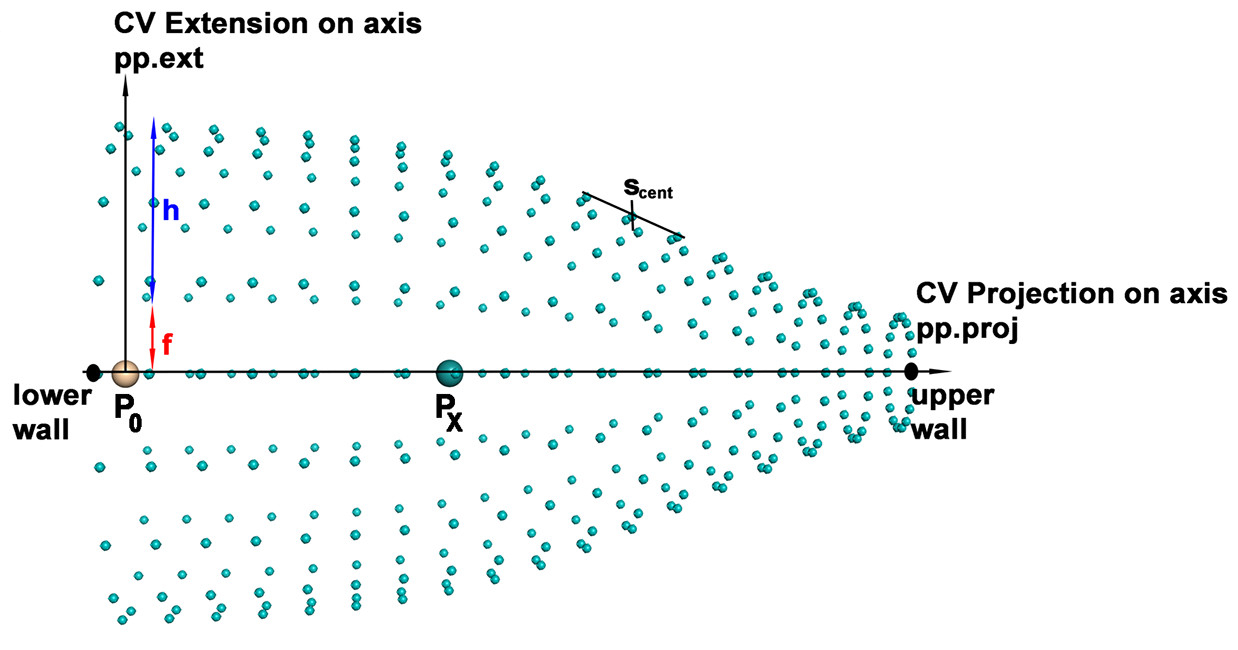
\includegraphics[width=\linewidth]{LIVECOMS/02_funnel_metad/funmetadfig1.jpeg}
\caption{Visualisation of the funnel restraints defined using the CV projection axis and the CV extent axis.}
\label{fig:funnel}
\end{figure}

The funnel parameters $h$ and $f$ controls the maximal and minimal width of the funnel along the extent axis respectively. The smoothness of the transition between maximal and minimal widths along the projection axis is controlled by the parameters $b$ and $x$ that together control the location and steepness of the inflection point located at $S_{cent}$ in fig \ref{fig:funnel}.  All together these parameters define the radius $S$ of the funnel at a given distance $i$ along the projection axis.  

\begin{equation}
S(i) = h\left(\frac{1}{1+b^{b(i-x)}}\right) + f,
\end{equation}

Clearly, there is still some degeneracy in the CVs - the plane
perpendicular to the projection axis is a one-dimensional representation of a two-dimensional space. However, this is a good compromise between having sufficient accuracy for describing the binding of a ligand and the tolerable simulation slowdown of using only two CVs.

In order to have a good separation between the bound and unbound phases for the ABFE estimations, the funnel needs to point \emph{out}, with the narrow end in the solvent,
and away from any protein residues. The BSS automated funnel assignment code does this generally well. Typically the vectors picked for defining the $P_{0}$ and $P_{1}$ points offer an unobstructed exit path for the ligand. It is nonetheless still a good idea to visually check the proposed funnel, especially for new protein systems. This can be done through use of the funnel visualisation functionality within BSS (see below).

The size of the funnel radius has to be determined on a case-by-case basis. The metadynamics code tracks the center of mass the ligand, therefore ligand atoms are able to sample positions outside the visualised funnel, provided the center of mass remains inside the funnel. the volume that the small molecule will explore is much larger than implied by the visualization of the funnel. There is usually only one binding site and the funnel should enclose only it, excluding other protein features, by setting a small value of $h$. This helps accelerate convergence by preventing the ligand from exploring irrelevant regions in the free energy surface (FES). 

\hypertarget{setupfunmetad}{%
\subsubsection{Setting up funnel metadynamics simulations}\label{setupfunmetad}}

The first tutorial notebook \href{https://github.com/OpenBioSim/biosimspace_tutorials/blob/main/02_funnel_metad/01_bss-fun-metad-setup.ipynb}{01-bss-fun-metad-setup} shows how to set up a BioSimSpace system, parameterizing the protein and the ligand, as well as defining the simulation box, adding water and ions. A funnel is then defined and visualized using NGLview. Finally, directories for the \emph{fun-metaD} simulation are setup and a short 10 ps simulation is run for illustrative purposes.


\begin{figure}[htp]
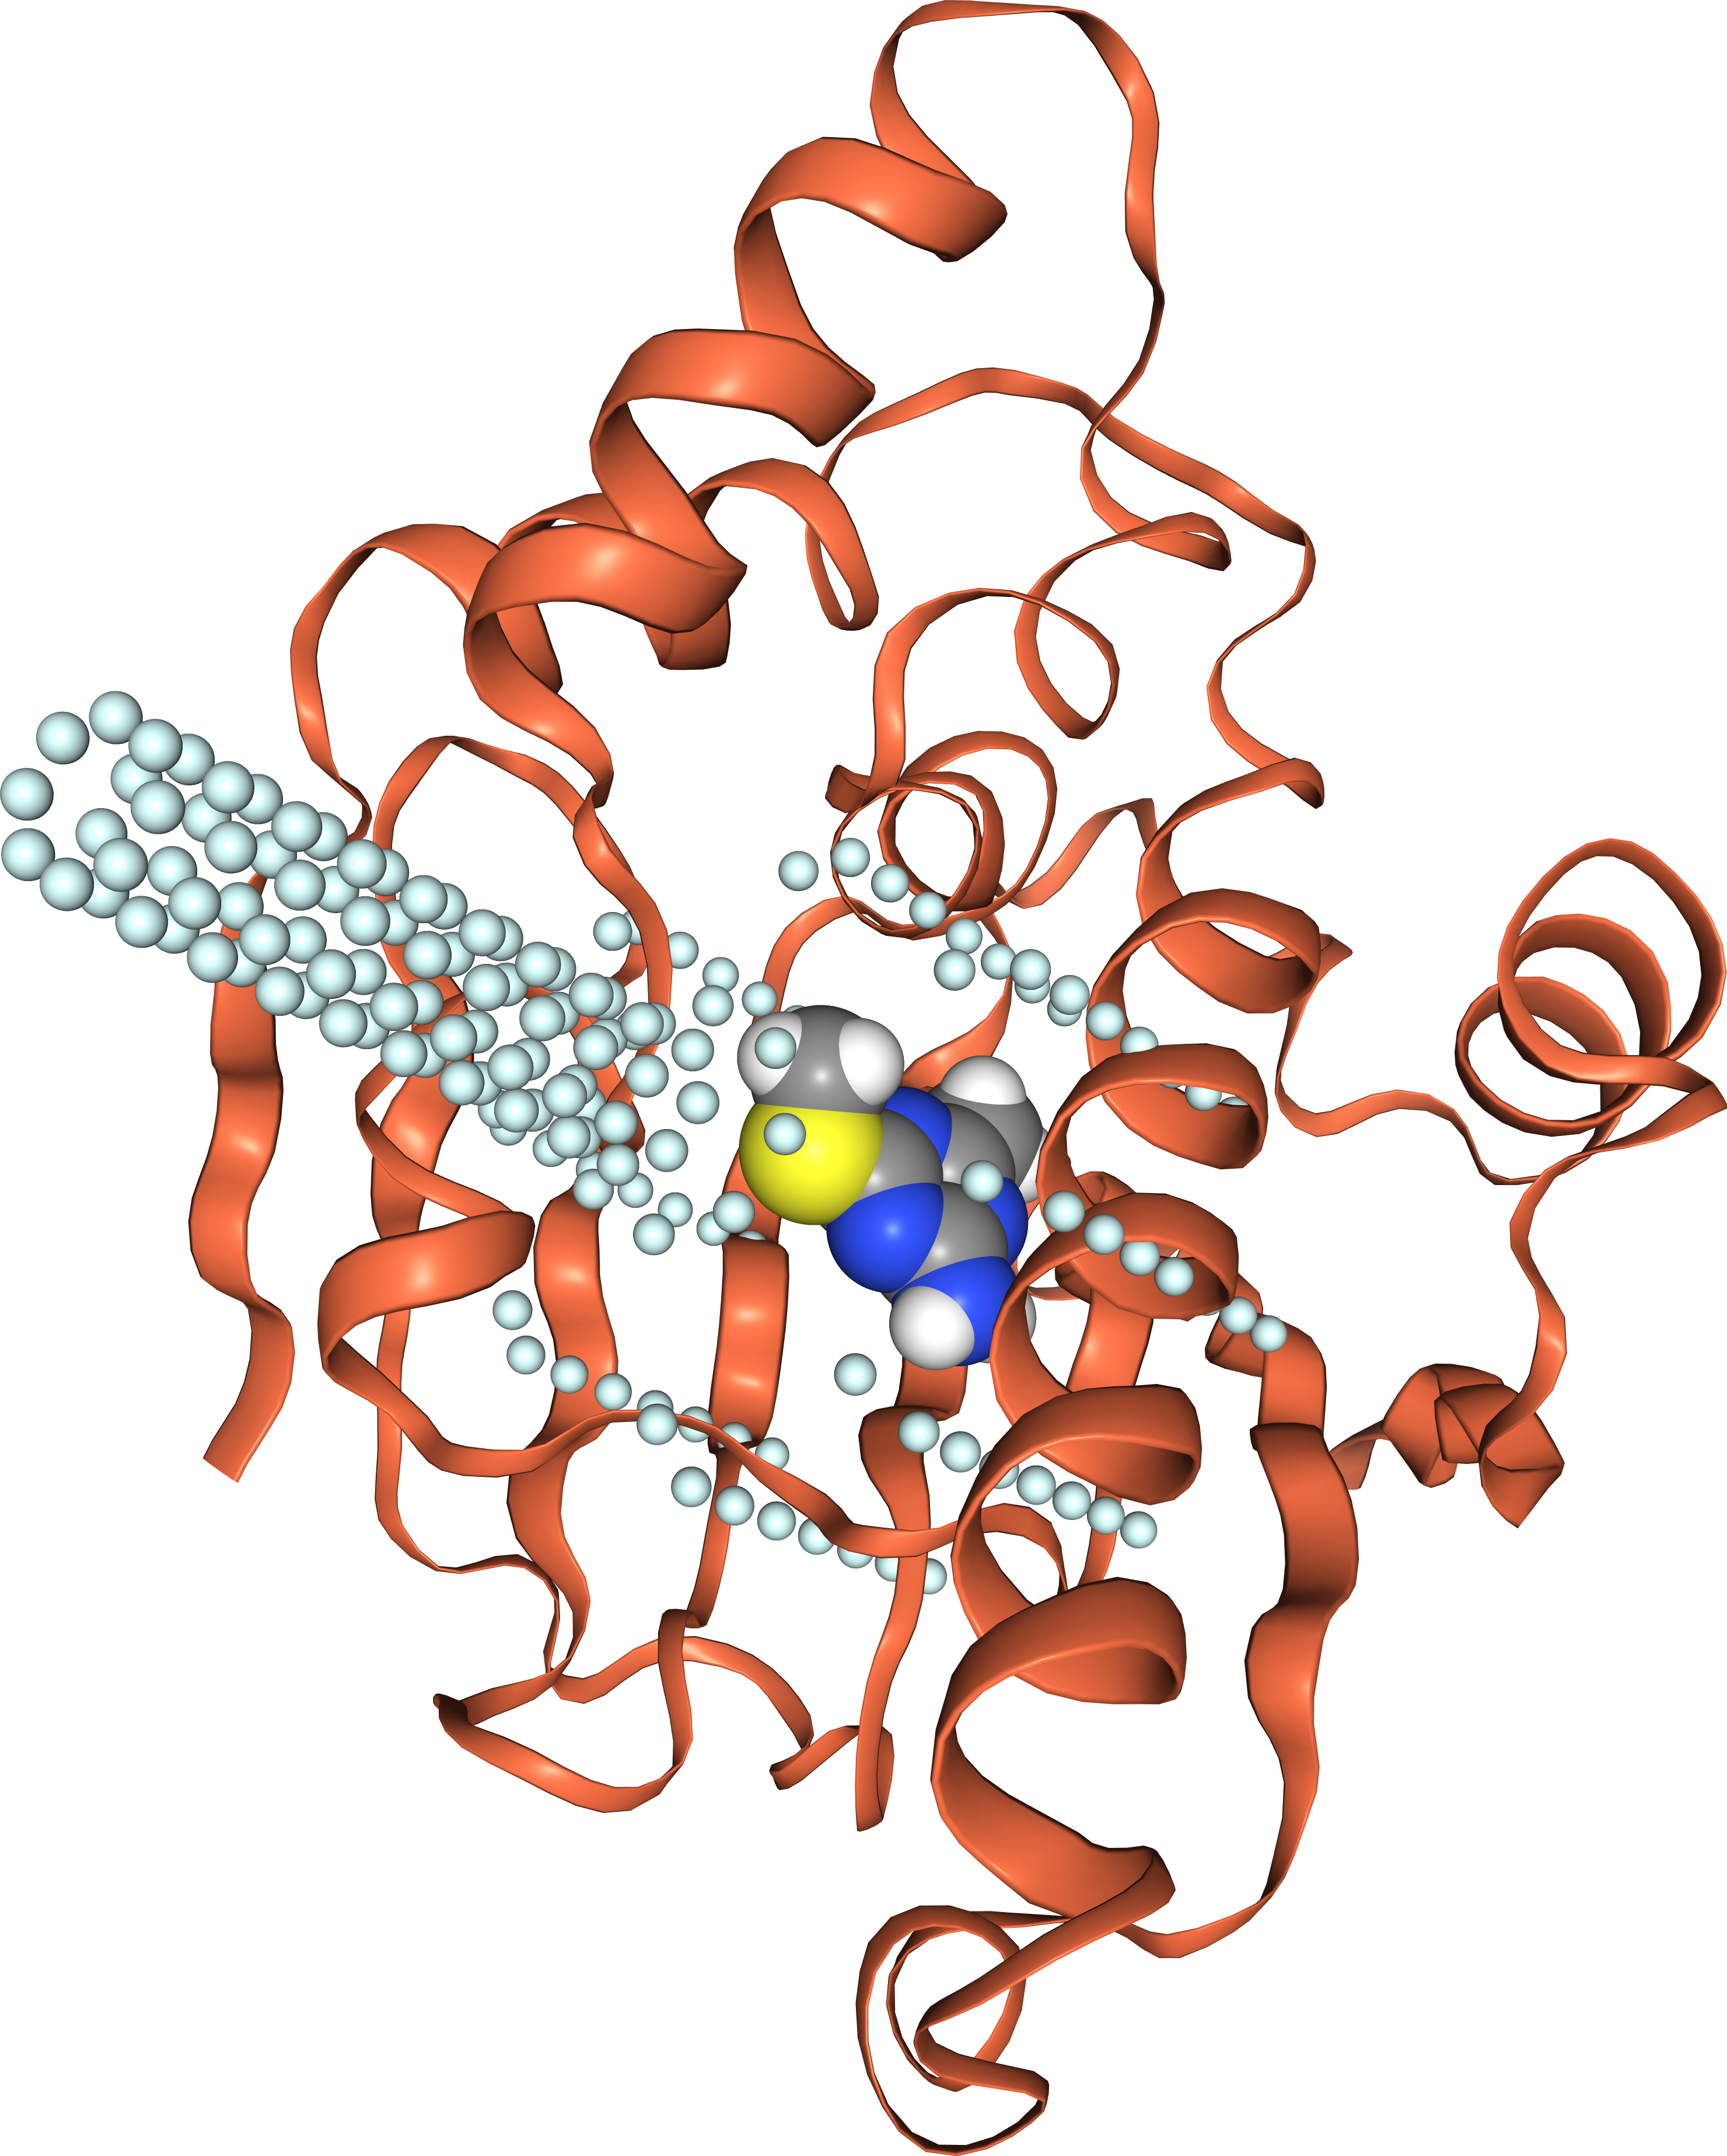
\includegraphics[width=\linewidth]{LIVECOMS/02_funnel_metad/funmetad-hsp90.png}
\caption{Visualisation of funnel restraints autogenerated by BioSimSpace for a HSP90 protein-ligand system.}
\label{fig:fun-hsp90}
\end{figure}

The notebook uses as example a fully solvated HSP90 protein-ligand system originally setup from PDBID:2WI2. 
Figure \ref{fig:fun-hsp90} depicts a rendered funnel overlayed on the HSP90 protein-ligand system in the Jupyter Notebook. The funnel vector is clearly pointing out into the solvent, with no protein residues blocking the way. The default radius is sufficient to encompass the binding site, excluding the rest of the protein.


To obtain converged free energies we recommend simulations of the order of 500 - 2000 ns sampling time. This is best done out of a notebook. For convenience we also \href{https://github.com/OpenBioSim/biosimspace_tutorials/tree/main/02_funnel_metad/example_nodes}{provide with this tutorial} as companion resource an LSF submission script that re-implements the notebook functionality in a set of BioSimSpace nodes.  

\hypertarget{analysis}{%
\subsubsection{Analysing funnel metadynamics simulations}\label{analysis}}

The second notebook of this tutorial  \href{https://github.com/OpenBioSim/biosimspace_tutorials/blob/main/02_funnel_metad/02_bss-fun-metad-analysis.ipynb}{02-bss-fun-metad-analysis} describes how to analyze a funnel metadynamics simulation. The precision of the ABFE estimate derived from a funnel metadynamics run is linked to the convergence of the free energy profile along the collective variables that define the funnel. The notebook uses provided sample trajectories to show how the range of CV values sampled during a trajectory and two-dimensional free energy surfaces can be plotted with the help of \href{https://biosimspace.openbiosim.org/api/index_Notebook.html}{BSS.Notebook}. The notebook also shows how to compute funnel correction terms using BSS, and how to perform convergence analysis of the absolute binding free energies for different trajectories. Selected visualizations generated by the notebook are depicted in Figure~\ref{fig:fun-hsp90-analyses}. 

\begin{figure}[htp]
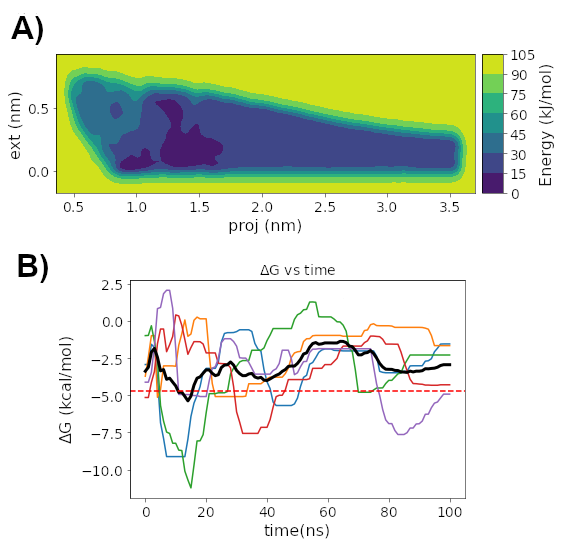
\includegraphics[width=\linewidth]{LIVECOMS/02_funnel_metad/fun-hsp90-analyses.png}
\caption{Selected analyses of funnel metadynamics simulations of the HSP90 protein-ligand system. A) Reconstructed two-dimensional free energy profile from a sample 100 ns trajectory. B) Convergence plots for five replicates of a 100-ns trajectory. The bold black line denotes the mean of the replicates, and the dashed red line the experimental estimate of the absolute binding free energy of the ligand.}
\label{fig:fun-hsp90-analyses}
\end{figure}



\subsection{Tutorial 3: Steered molecular dynamics}
\subsubsection{Introduction}
Many relevant biological processes, such as transmembrane permeation or transitions between active and inactive protein conformations, occur on a timescale of $\mu$ s-s~\cite{Zwier2010,Choy2017,Wells2007}. However, even with GPU acceleration, the timescales accessible via MD simulations are only a few hundred ns/day~\cite{HecBioSim_benchmark}. One of the methods to get around this limitation is steered molecular dynamics (sMD). sMD involves applying a harmonic restraint to bias the system towards a conformation defined through one or more collective variables (CVs):

\begin{equation}
V(\vec{s},t) = \frac{1}{2} \kappa(t) ( \vec{s} - \vec{s}_0(t) )^2,
\label{eq:sMD}
\end{equation}

where $\kappa$ is the force constant, $\vec{s}_0$ is the expected CV value at a specific timestep, and $\vec{s}$ is the actual CV value at that timestep\cite{Isralewitz2001,Tribello2014}.

This section of the tutorial summarizes how to use BioSimSpace to set up and run sMD simulations. BSS prepares input files for PLUMED, which is the software that works together with MD engines such as AMBER and GROMACS to add the restraint in eq~\ref{eq:sMD}.

We use protein tyrosine phosphatase 1B (PTP1B) as the system of choice for this tutorial. It is a negative regulator of insulin signalling~\cite{sMD_ptp1b-diabetes} and is an attractive target for type II diabetes~\cite{sMD_Wiesman}. The function of PTP1B depends on the conformation of its WPD loop, which can be closed (active) or open (inactive) (Figure~\ref{fig:ptp1b}). The WPD loop of PTP1B opens and closes on a $\mu$s timescale~\cite{Choy2017}, and therefore this transition is not observed on conventional computational timescales.

\begin{figure}[htp]
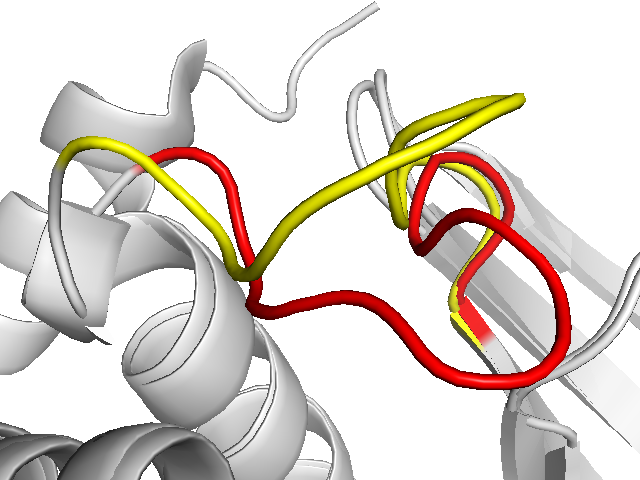
\includegraphics[width=\linewidth]{LIVECOMS/03_steered_md/open-close.png}
\caption{The WPD loop of PTP1B, in two conformations: open (yellow, PDB ID: 2HNP) and closed (red, PDB ID: 1SUG).}
\label{fig:ptp1b}
\end{figure}

\subsubsection{Running sMD using BioSimSpace}

The first notebook of this tutorial \href{https://github.com/OpenBioSim/biosimspace_tutorials/blob/main/03_steered_md/01_setup_sMD.ipynb}{01-setup-sMD} describes how to set up a steered MD simulation with BioSimSpace. 
The notebook illustrates the use of \href{https://biosimspace.openbiosim.org/api/generated/BioSimSpace.Metadynamics.CollectiveVariable.RMSD.html#BioSimSpace.Metadynamics.CollectiveVariable.RMSD}{BSS.Metadynamics.CollectiveVariable.RMSD} to define a collective variable that enforces a conformational change of the 'WPD' loop in the enzyme PTP1B. 
Next \href{https://biosimspace.openbiosim.org/api/generated/BioSimSpace.Protocol.Steering.html#BioSimSpace.Protocol.Steering}{BSS.Protocol.Steering} is used to specify a steering schedule alongside the RMSD CV. The notebook illustrates how input files for the \emph{gmx}, \emph{sander} or \emph{pmemd} MD engines can be subsequently prepared. The notebook also shows how a more complex steering schedule that combines multiple CVs can be written. 

For production simulations, we recommend long sMD simulations to minimize the strength of the bias that needs to be applied to enforce the desired conformational change by the end of the steered MD simulation. Optimizing the steered MD schedule parameters requires trial and error. 
For convenience, we provide simple Python scripts with a command line interface to execute steered MD runs and scan schedule parameters for two specified sMD protocols (\href{https://github.com/OpenBioSim/biosimspace_tutorials/blob/main/03_steered_md/scripts/sMD_simple.py}{a single CV} and a \href{https://github.com/OpenBioSim/biosimspace_tutorials/blob/main/03_steered_md/scripts/sMD_multiCV.py}{multiple CV} example). We also provide sample \href{https://github.com/OpenBioSim/biosimspace_tutorials/blob/main/03_steered_md/scripts/sMD_slurm.sh}{slurm} and \href{https://github.com/OpenBioSim/biosimspace_tutorials/blob/main/03_steered_md/scripts/sMD_LSF.sh}{LSF} submission scripts to deploy the BSS steered MD scripts in different HPC environments. 

\subsubsection{sMD trajectory analysis}

The second notebook of this tutorial \href{https://github.com/OpenBioSim/biosimspace_tutorials/blob/main/03_steered_md/02_trajectory_analysis.ipynb}{02-trajectory-analysis} describes how to analyze data generated by a steered MD run. As the sMD simulation is run, the CV values are saved to a \textbf{COLVAR} file. It can be plotted to assess whether the sMD simulation has been successful. An example is shown in Figure \ref{fig:rmsd}.

\begin{figure}[htp]
    \centering
    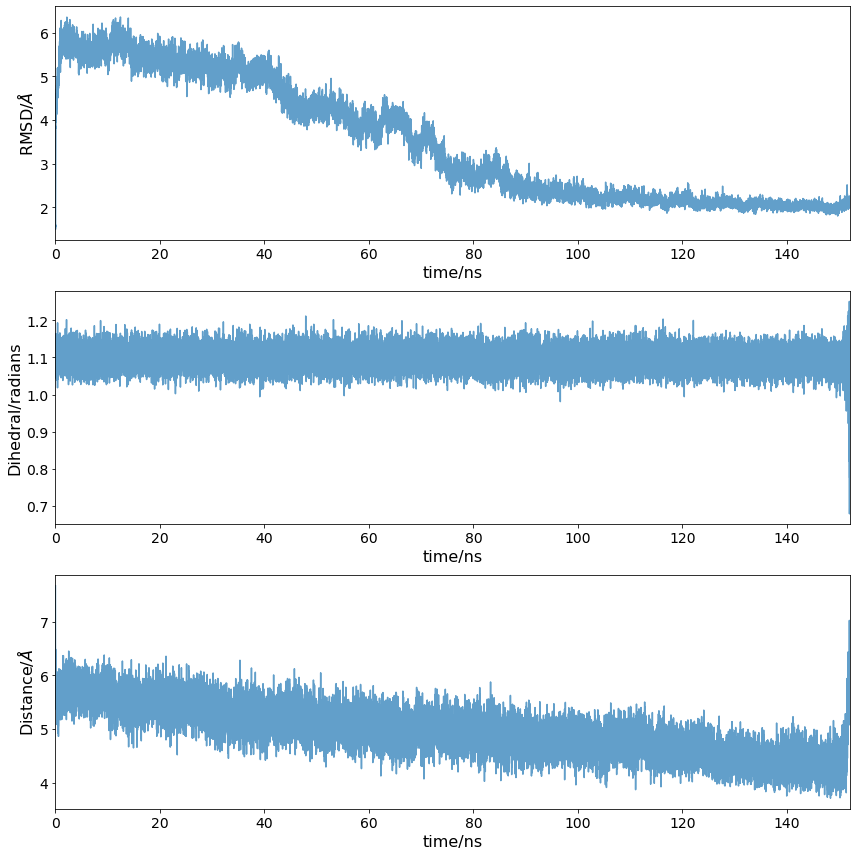
\includegraphics[width=\linewidth]{LIVECOMS/03_steered_md/COLVAR_all.png}
    \caption{Evolution of Collective Variables throughout an sMD simulation. A) RMSD CV measuring distance to closed WPD loop conformation. B) Torsional angle CV measuring the Chi1 angle of residue Tyr 152. C)  CV measuring the distance between C$_{\gamma}$ atoms in residues Phe196 and Phe280. As the simulation progresses, the WPD loop RMSD is gradually lower (i.e. the loop is adopting a  closed loop conformation).}
    \label{fig:rmsd}
\end{figure}

The notebook also illustrates a "failed" steered MD trajectory, where the steering duration and force were insufficient to reach the target CV value.

\subsubsection{Markov State Models}
While the information provided here focuses on running sMD simulations with BSS, there are multiple potential applications, such as studying membrane permeability~\cite{Wells2007} or ligand residence time\cite{Potterton2019}. Another use is for the additional exploration of conformational space for predicting allosteric modulation using Markov State Models (MSMs). MSMs give the probability of protein conformations and therefore can be used to model how a ligand affects the conformation ensemble of a target (e.g. whether it decreases the active state probability and therefore is an allosteric inhibitor). There is a lot to consider when building MSMs, and the method is not covered in this tutorial. Here the Python library \href{http://emma-project.org/latest/}{PyEMMA} was used, which has extensive examples and documentation\cite{Wehmeyer_2019}. The integration of sMD in this allosteric modulation prediction workflow is illustrated in Figure \ref{fig:ensemble-protocol}. \href{https://github.com/OpenBioSim/BioSimSpaceTutorials/blob/main/03_steered_md/02_trajectory_analysis.ipynb}{02-trajectory-analysis} shows how the sMD trajectory can be sampled to extract a range of protein conformations. Hardie \emph{et al} report a detailed study of allosteric modulators of PTP1B using this sMD/MSM methodology~\cite{Hardie2023}.

\begin{figure}[htp]
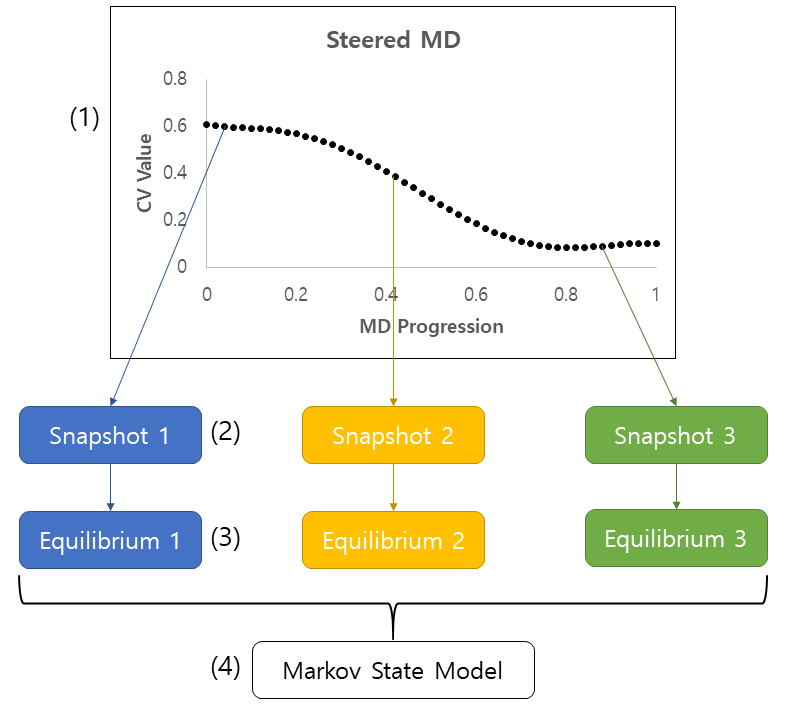
\includegraphics[width=\linewidth]{LIVECOMS/03_steered_md/ensemble-md-protocol.png}
\caption{The steps used for enhanced sampling methods to gather data for statistical analysis of protein conformation ensemble. (1) Run steered MD along some collective variable (CV); (2) Extract snapshots that evenly sample available conformational space; (3) Run equilibrium MD simulations using extracted coordinates as seeds; (4) construct an MSM using trajectory data from step 3.}
\label{fig:ensemble-protocol}
\end{figure}

\subsection{Tutorial 4: Alchemical free energy calculations}
%%%%%%%%%%%%%%%%%%%%%%%%%%%%%%%%%%%%%%%%%%%%%%%%%%%%%%%%%%%%%%%%%%%%%%%%%%%%%%%%%%%%%%%%%%%
%%%%%%%%%%%%%%%%%%%%%%%%%%%%%%%%%%%%%%%%%%%%%%%%%%%%%%%%%%%%%%%%%%%%%%%%%%%%%%%%%%%%%%%%%%%
%%%%%%%%%%%%%%%%%%%%%%%%%%%%%%%%%%%%%%%%%%%%%%%%%%%%%%%%%%%%%%%%%%%%%%%%%%%%%%%%%%%%%%%%%%%
%%%%%%%%%%%%%%%%%%%%%%%%%%%%%%%%%%%%%%%%%%%%%%%%%%%%%%%%%%%%%%%%%%%%%%%%%%%%%%%%%%%%%%%%%%%
%%%%%%%%%%%%%%%%%%%%%%%%%%%%%%%%%%%%%%%%%%%%%%%%%%%%%%%%%%%%%%%%%%%%%%%%%%%%%%%%%%%%%%%%%%%
%%%%%%%%%%%%%%%%%%%%%%%%%%.  WRITE YOUR CHAPTER CONTENTS BELOW.  %%%%%%%%%%%%%%%%%%%%%%%%%%
%%%%%%%%%%%%%%%%%%%%%%%%%%%%%%%%%%%%%%%%%%%%%%%%%%%%%%%%%%%%%%%%%%%%%%%%%%%%%%%%%%%%%%%%%%%
%%%%%%%%%%%%%%%%%%%%%%%%%%%%%%%%%%%%%%%%%%%%%%%%%%%%%%%%%%%%%%%%%%%%%%%%%%%%%%%%%%%%%%%%%%%
%%%%%%%%%%%%%%%%%%%%%%%%%%%%%%%%%%%%%%%%%%%%%%%%%%%%%%%%%%%%%%%%%%%%%%%%%%%%%%%%%%%%%%%%%%%

\subsubsection{Introduction}


Computational chemists can support the study of structure-activity relationships in medicinal chemistry by making computer models that can predict the binding affinity of ligands to proteins. Alchemical free energy (AFE) methods are a popular class of methodologies to do so. Some
introductory reading is recommended ~\cite{mey2020best, cournia_allen_sherman_2017, kuhn_firth-clark_tosco_mey_mackey_michel_2020, Hahn2022}.

This tutorial covers the basic principles of alchemical free energy calculations with BioSimSpace; how to setup, simulate, and analyze alchemical Relative Binding Free Energy (RBFE) calculations for congeneric series of protein-ligand complexes; how to set up and analyze alchemical ABFE calculations of a ligand bound to a protein.  
The notebooks prompt the readers to complete a series of exercises that typically involve completing cells to test their understanding of the material presented. 

\subsubsection{Setting up AFE calculations using BioSimSpace}

The first notebook of this tutorial \href{https://github.com/OpenBioSim/biosimspace_tutorials/blob/main/04_fep/01_intro_to_alchemy/alchemical_introduction.ipynb}{alchemical-introduction} introduces the basic functionality available in BioSimSpace to implement AFE calculations. 
The notebook first introduces the functionality of the \href{https://biosimspace.openbiosim.org/api/index_Align.html}{BSS.Align} module. BSS.Align implements a variety of mapping algorithms based on maximum common substructure searches between a supplied pair of molecules to generate a 'merged' molecule used to describe an alchemical transformation. This is used to generate a merged molecule that describes the alchemical transformation of ethane into methanol.
Next, the use of \href{https://biosimspace.openbiosim.org/api/generated/BioSimSpace.Protocol.FreeEnergy.html#BioSimSpace.Protocol.FreeEnergy}{BSS.Protocol.FreeEnergy} is illustrated using the relative hydration free energy of ethanol to methane as an example, using the AFE engines \emph{SOMD} \cite{Calabr2016} or \emph{mdrun}. 
The AFE simulations can in principle be executed directly from the notebook as a set of independent MD simulations run serially, but this is often too slow to be practical. The next section describes protocols to submit calculations in parallel on HPC resources.
Finally, the notebook describes the setup of the relative binding free energy calculation of benzene to o-xylene bound to the protein T4 lyzozyme mutant. 
\\
The notebook then describes the use of \href{https://biosimspace.openbiosim.org/api/generated/BioSimSpace.FreeEnergy.Relative.html#}{BSS.FreeEnergy.Relative} to process the completed AFE simulations for two legs of a thermodynamic cycle using MBAR or TI to obtain a free energy estimate. The resulting free energy changes are subtracted to yield a relative binding free energy for o-xylene to benzene. Finally, the plotting of overlap matrices is demonstrated to assess the reliability of a computed free energy change. The functionality covered by this notebook is illustrated in Figure \ref{thermodynamic_cycle_fig}.

\begin{figure}[htp]
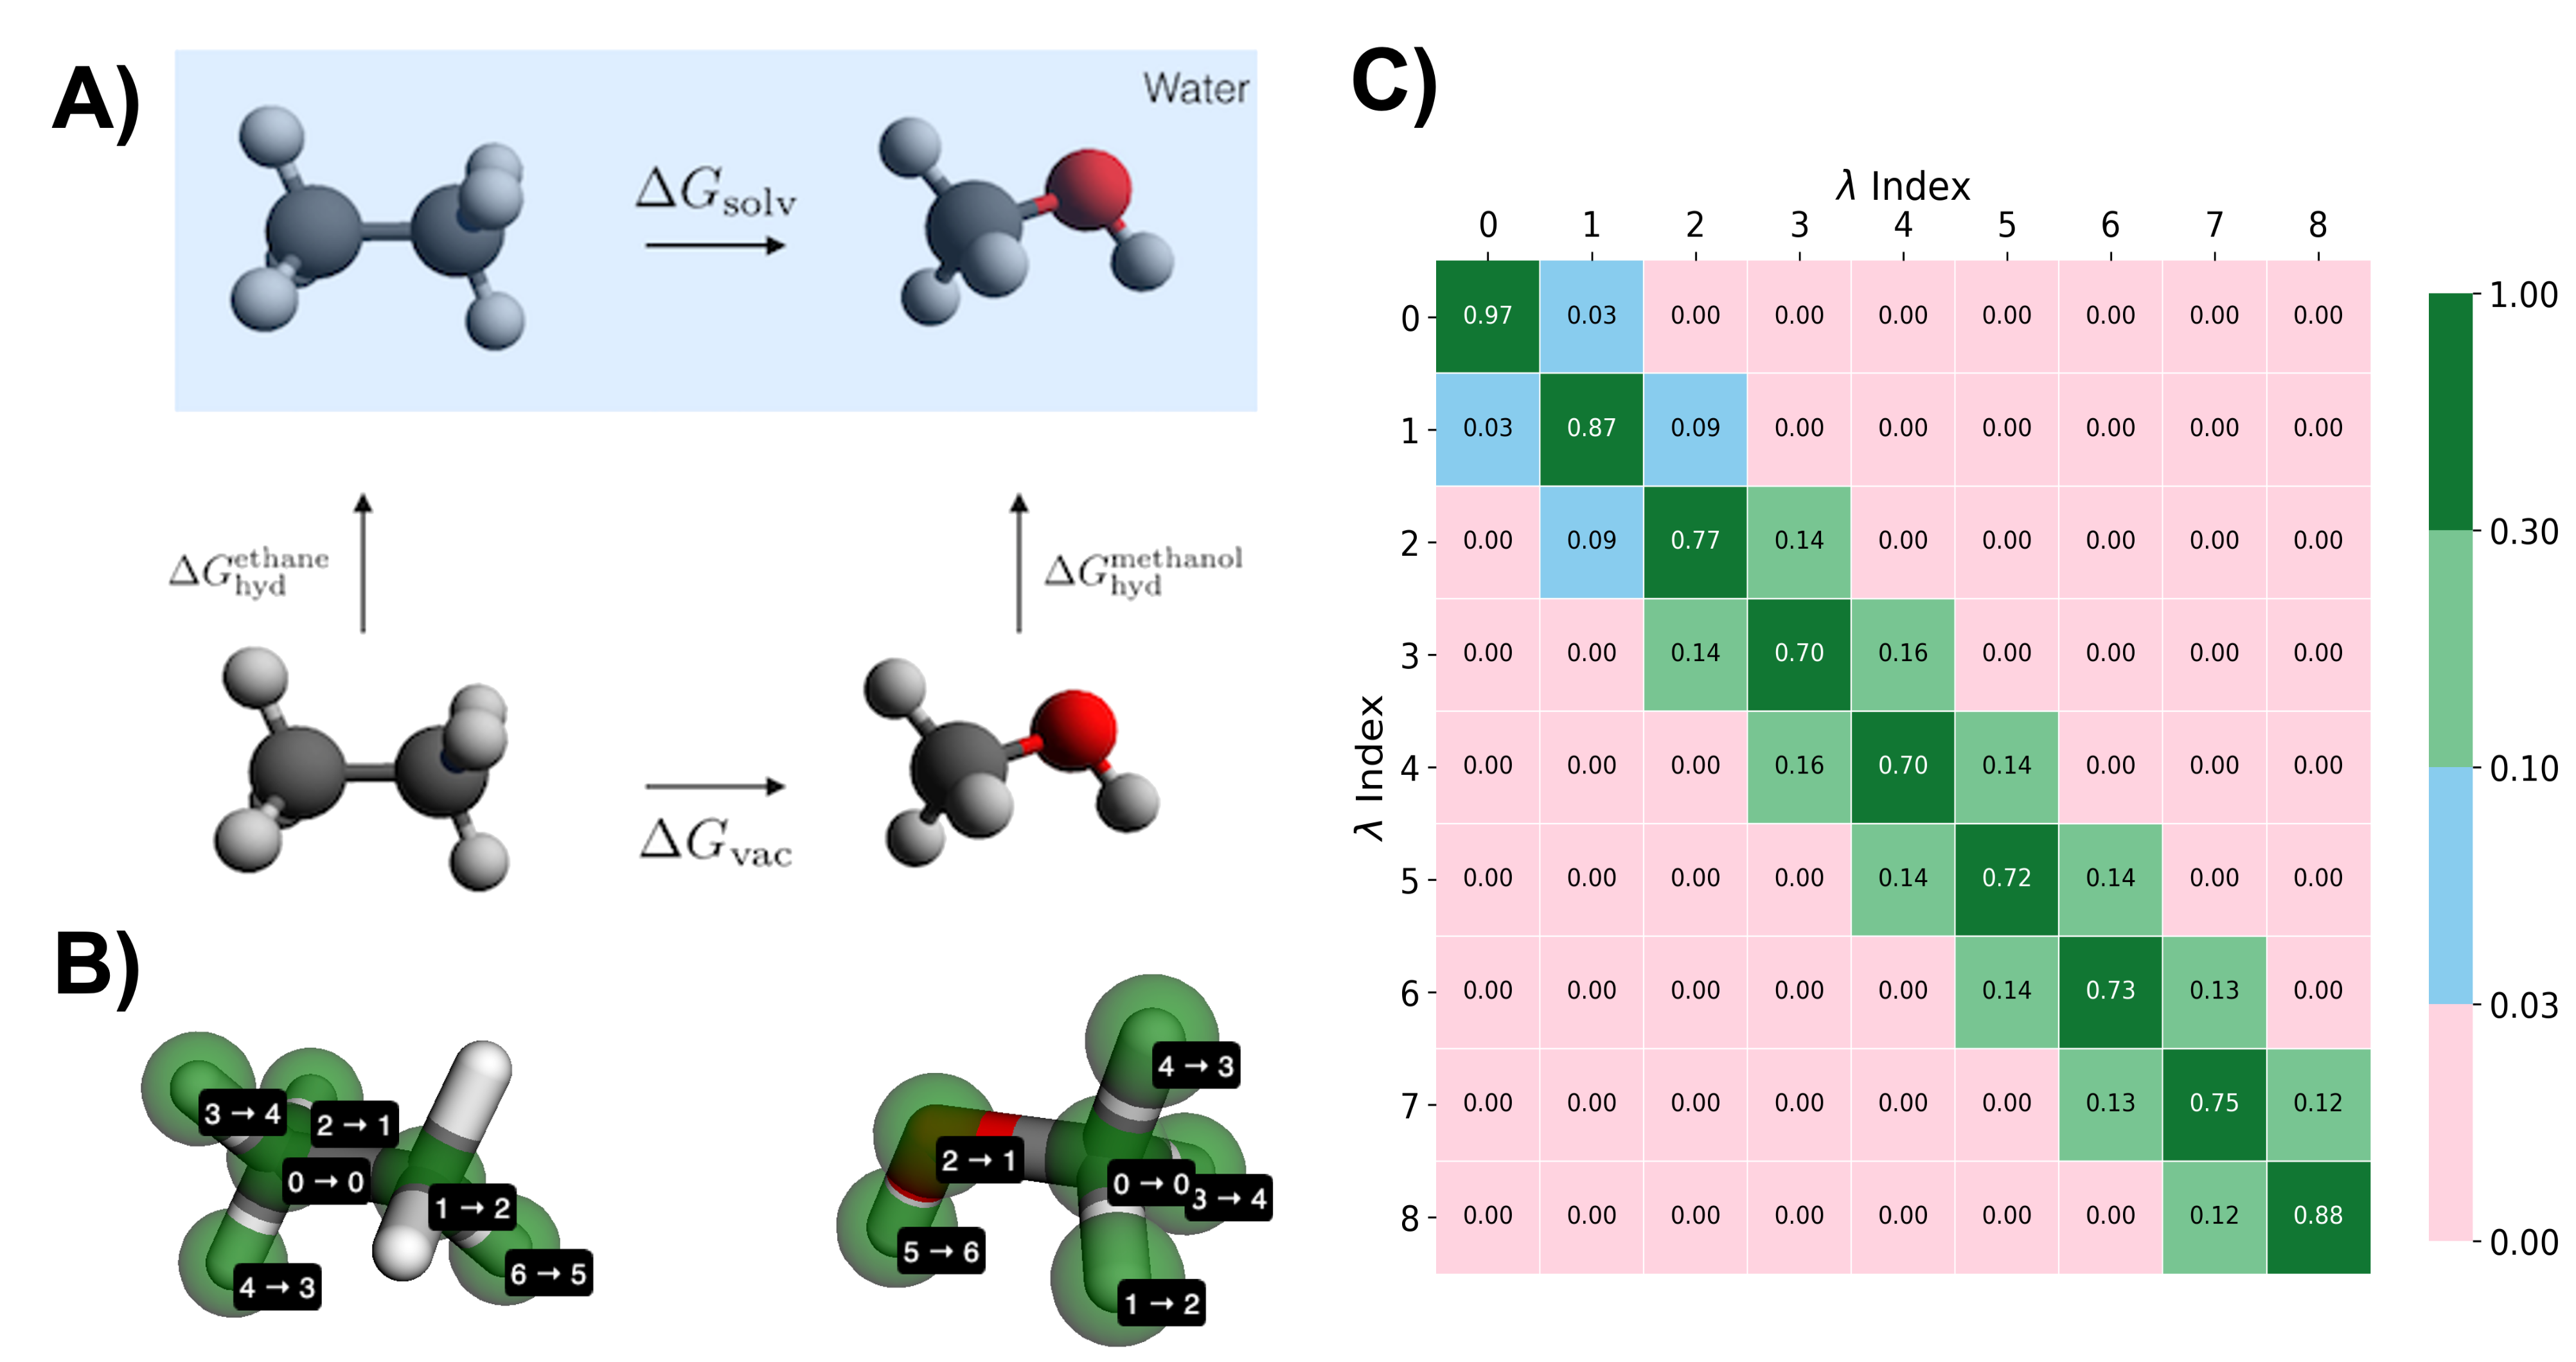
\includegraphics[width=\linewidth]{LIVECOMS/04_fep/introfep_updated.png}
\caption{ \textbf{A)} Thermodynamic cycle used to compute the relative hydration free energy of ethane to methanol. \textbf{B)} Visualisation of the atom mappings between ethane and methanol generated by \emph{BSS.Align}. \textbf{C)} Visualisation of overlap matrix generated by \emph{BSS.Notebook.plotOverlapMatrix} to help assess the reliability of a calculated free energy change.}
\label{thermodynamic_cycle_fig}
\end{figure}


\subsubsection{RBFE calculation pipelines}

The second notebook of this tutorial \href{https://github.com/OpenBioSim/biosimspace_tutorials/blob/main/04_fep/02_RBFE/01_setup_rbfe.ipynb}{01-setup-rbfe.ipynb} shows how to design an RBFE campaign for a congeneric series of protein-ligand complexes. This is illustrated using a dataset of ligands for the protein TYK2, taken from the benchmark set of Wang et al. \cite{Wang2015} 
First, a drop-down menu is presented to the user to enable the selection of a variety of configuration settings (such as the choice of forcefields to use for the ligands, the protein, or the FEP engine to select). In BSS 2023.3.0 the FEP engines \emph{SOMD} and \emph{mdrun} (from the GROMACS software suite) are supported. An \href{https://github.com/michellab/BioSimSpace/tree/feature-amber-fep}{experimental feature branch} that implements support for RBFE calculations with the MD engine pmemd from the AMBER software suite is also available. 

Next, \href{https://biosimspace.openbiosim.org/api/generated/BioSimSpace.Align.generateNetwork.html}{BSS.Align.generateNetwork} is used to interface with the LOMAP software~\cite{Liu2013} to propose a network of relative transformations that span the provided ligand dataset. The notebook illustrates interactive plotting of the proposed network and how to make manual adjustments such as adding or deleting edges or inserting new ligands into the network. Once the user is satisfied with the chosen FEP network, setup instructions are saved to disk. 
\\
Processing the entire TYK2 dataset involves setting up and running several hundred MD simulations of solvated ligands and protein-ligand complexes. This would be impractically slow if executed from a notebook on a single workstation. For convenience, we provide a sample \href{https://github.com/OpenBioSim/biosimspace_tutorials/blob/main/04_fep/02_RBFE/scripts/run_all_slurm.sh}{slurm submission script} that processes the setup, simulation and analysis of the entire network constructed by the RBFE setup notebook on an HPC environment. This script may be adjusted for deployment on different slurm clusters or as reference for the implementation of the execution model on different schedulers. The functionality covered by this notebook is illustrated in Figure \ref{rbfe_setup_fig}.
\\

\begin{figure}[htp]
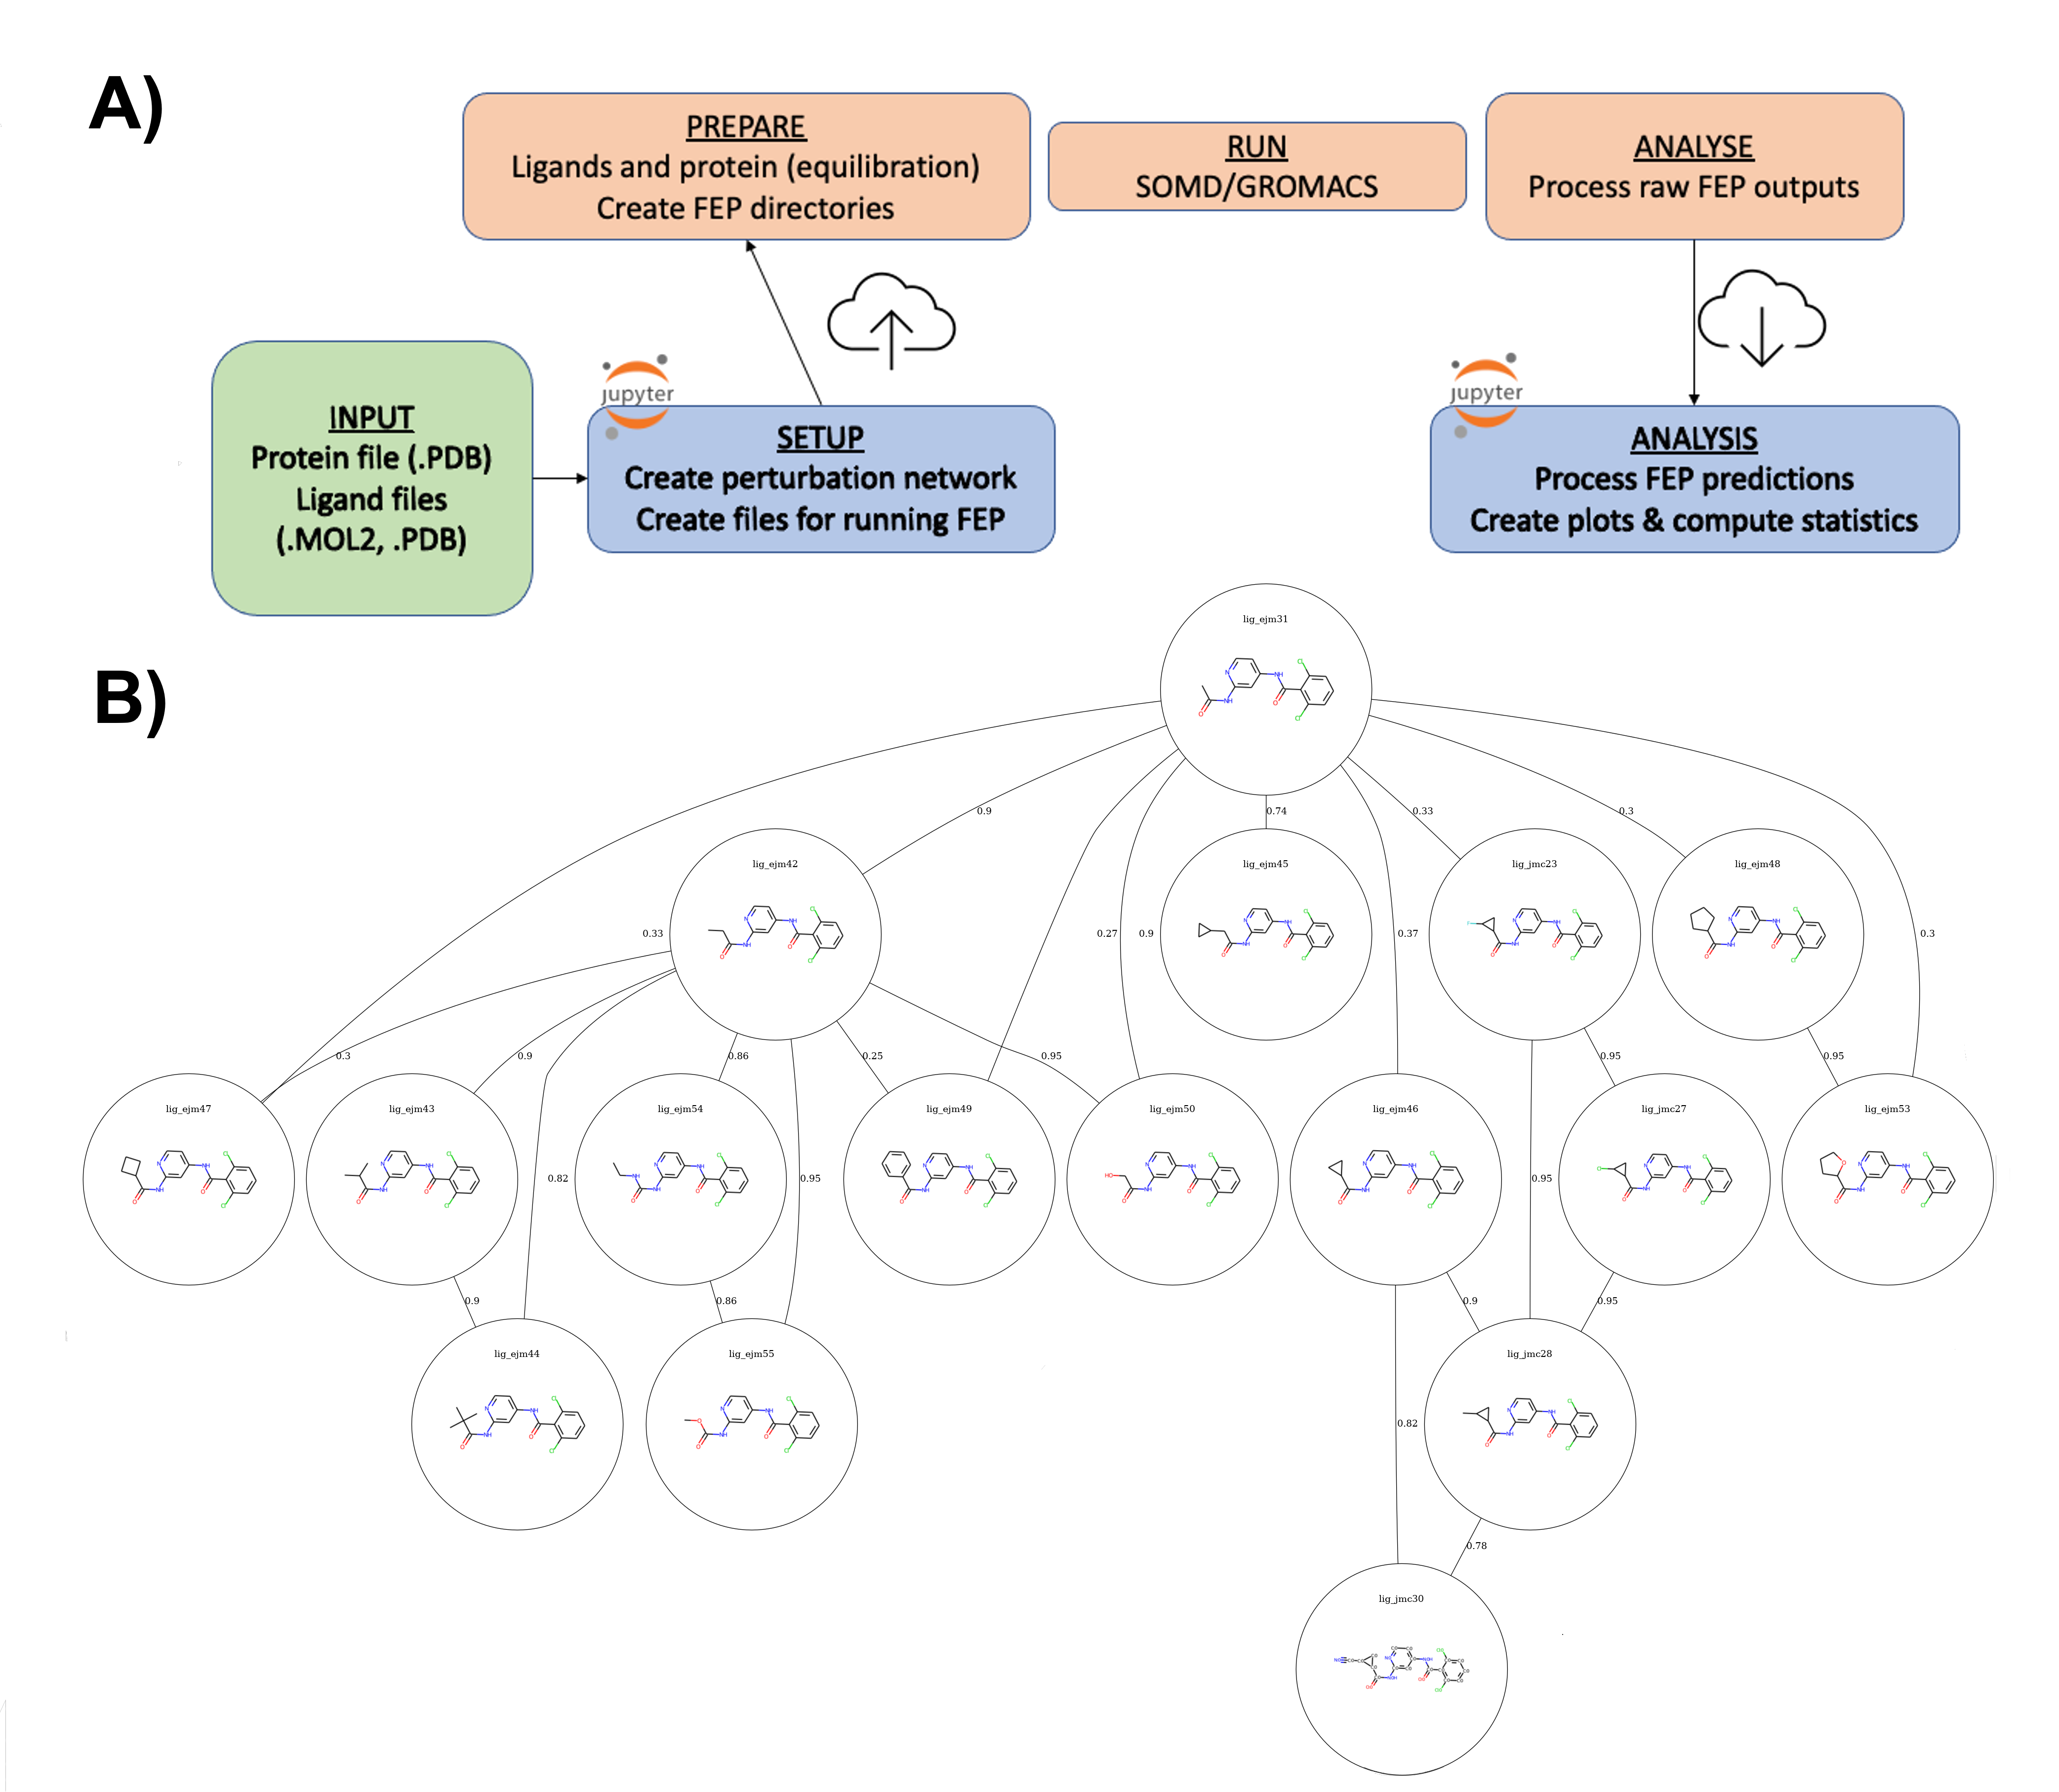
\includegraphics[width=\linewidth]{LIVECOMS/04_fep/rbfe-setup.png}
\caption{ \textbf{A)} Schematic of the RBFE pipeline in this tutorial. Whereas blue boxes represent notebooks run on a local machine, orange boxes represent Python scripts run sequentially on a computing cluster.
\textbf{B)} Perturbation network proposed by \emph{BSS.Align.generateNetwork} for a dataset of TYK2 ligands.} 
\label{rbfe_setup_fig}
\end{figure}


The third notebook \href{https://github.com/OpenBioSim/biosimspace_tutorials/blob/main/04_fep/02_RBFE/02_analysis_rbfe.ipynb}{02-analysis-rbfe} provides a walk-through of the analysis of the processed RBFE network. 
The RBFE network is first visualized using \emph{NetworkX}. Next, mean relative binding free energies are evaluated for each edge by averaging the results from all replicates available for each edge. The standard error of the mean is used as an estimate of the statistical uncertainty of each edge RBFE. A scatter plot comparing relative vs calculated binding free energies is produced, this is only possible because experimental data is available for this dataset. 
\\
Next, the set of RBFEs is converted into a set of binding free energies with an arbitrary reference value using the \emph{cinnabar} software to produce a scatter plot of calculated vs experimental binding free energies, together with statistical measures of accuracy (mean unsigned error, root mean squared error, Pearson coefficient, and Kendall tau coefficient). The functionality covered by this notebook is illustrated in Figure \ref{rbfe_analysis_fig}.
\\

\begin{figure}[htp]
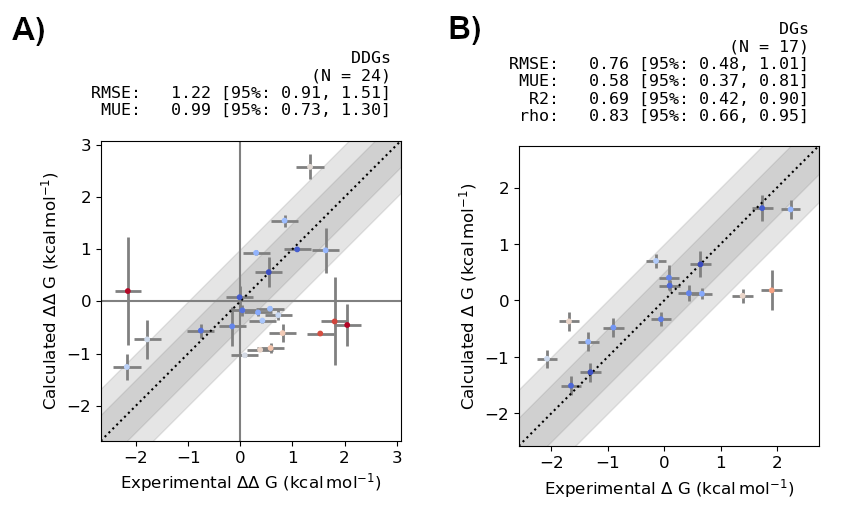
\includegraphics[width=\linewidth]{LIVECOMS/04_fep/rbfe-analysis.png}
\caption{ \textbf{A)} Scatter plot of experimental vs computed pairwise $\Delta \Delta G_{bind}$ free energies from the analysed perturbation network. \textbf{B)} Scatter plot of $\Delta G_{bind}$ estimates after processing of the network. } 
\label{rbfe_analysis_fig}
\end{figure}

\subsubsection{ABFE calculations}
%
The fourth notebook \href{https://github.com/OpenBioSim/biosimspace_tutorials/blob/main/04_fep/03_ABFE/01_setup_abfe.ipynb}{01-setup-abfe} describes how to set up alchemical ABFE calculations with BSS for use with either \emph{mdrun} or \emph{SOMD}. This free energy functionality is currently implemented in Exscientia's sandpit area of this version of BioSimSpace. Sandpits are used to test experimental features without accidentally breaking core functionality of the toolkit. 

Although RBFE calculations can be very useful in drug discovery, several important problems lie outside the scope of standard RBFE calculations. These include the calculation of the binding free energies of structurally dissimilar ligands to a common target; the calculation of the binding free energies of the same ligand to the same protein with different binding poses; the calculation of the binding free energies of a single ligand to a range of targets, as would be required to optimize selectivity or promiscuity. These quantities can be calculated using alchemical ABFE calculations because they utilize a more general \emph{double decoupling} thermodynamic cycle than in RBFE calculations \cite{gilson_statistical-thermodynamic_1997}. This involves entirely removing the ligand's intermolecular interactions in the presence of restraints between the ligand and receptor, as shown in Figure \ref{abfe_fig}A. 

\begin{figure}[htp]
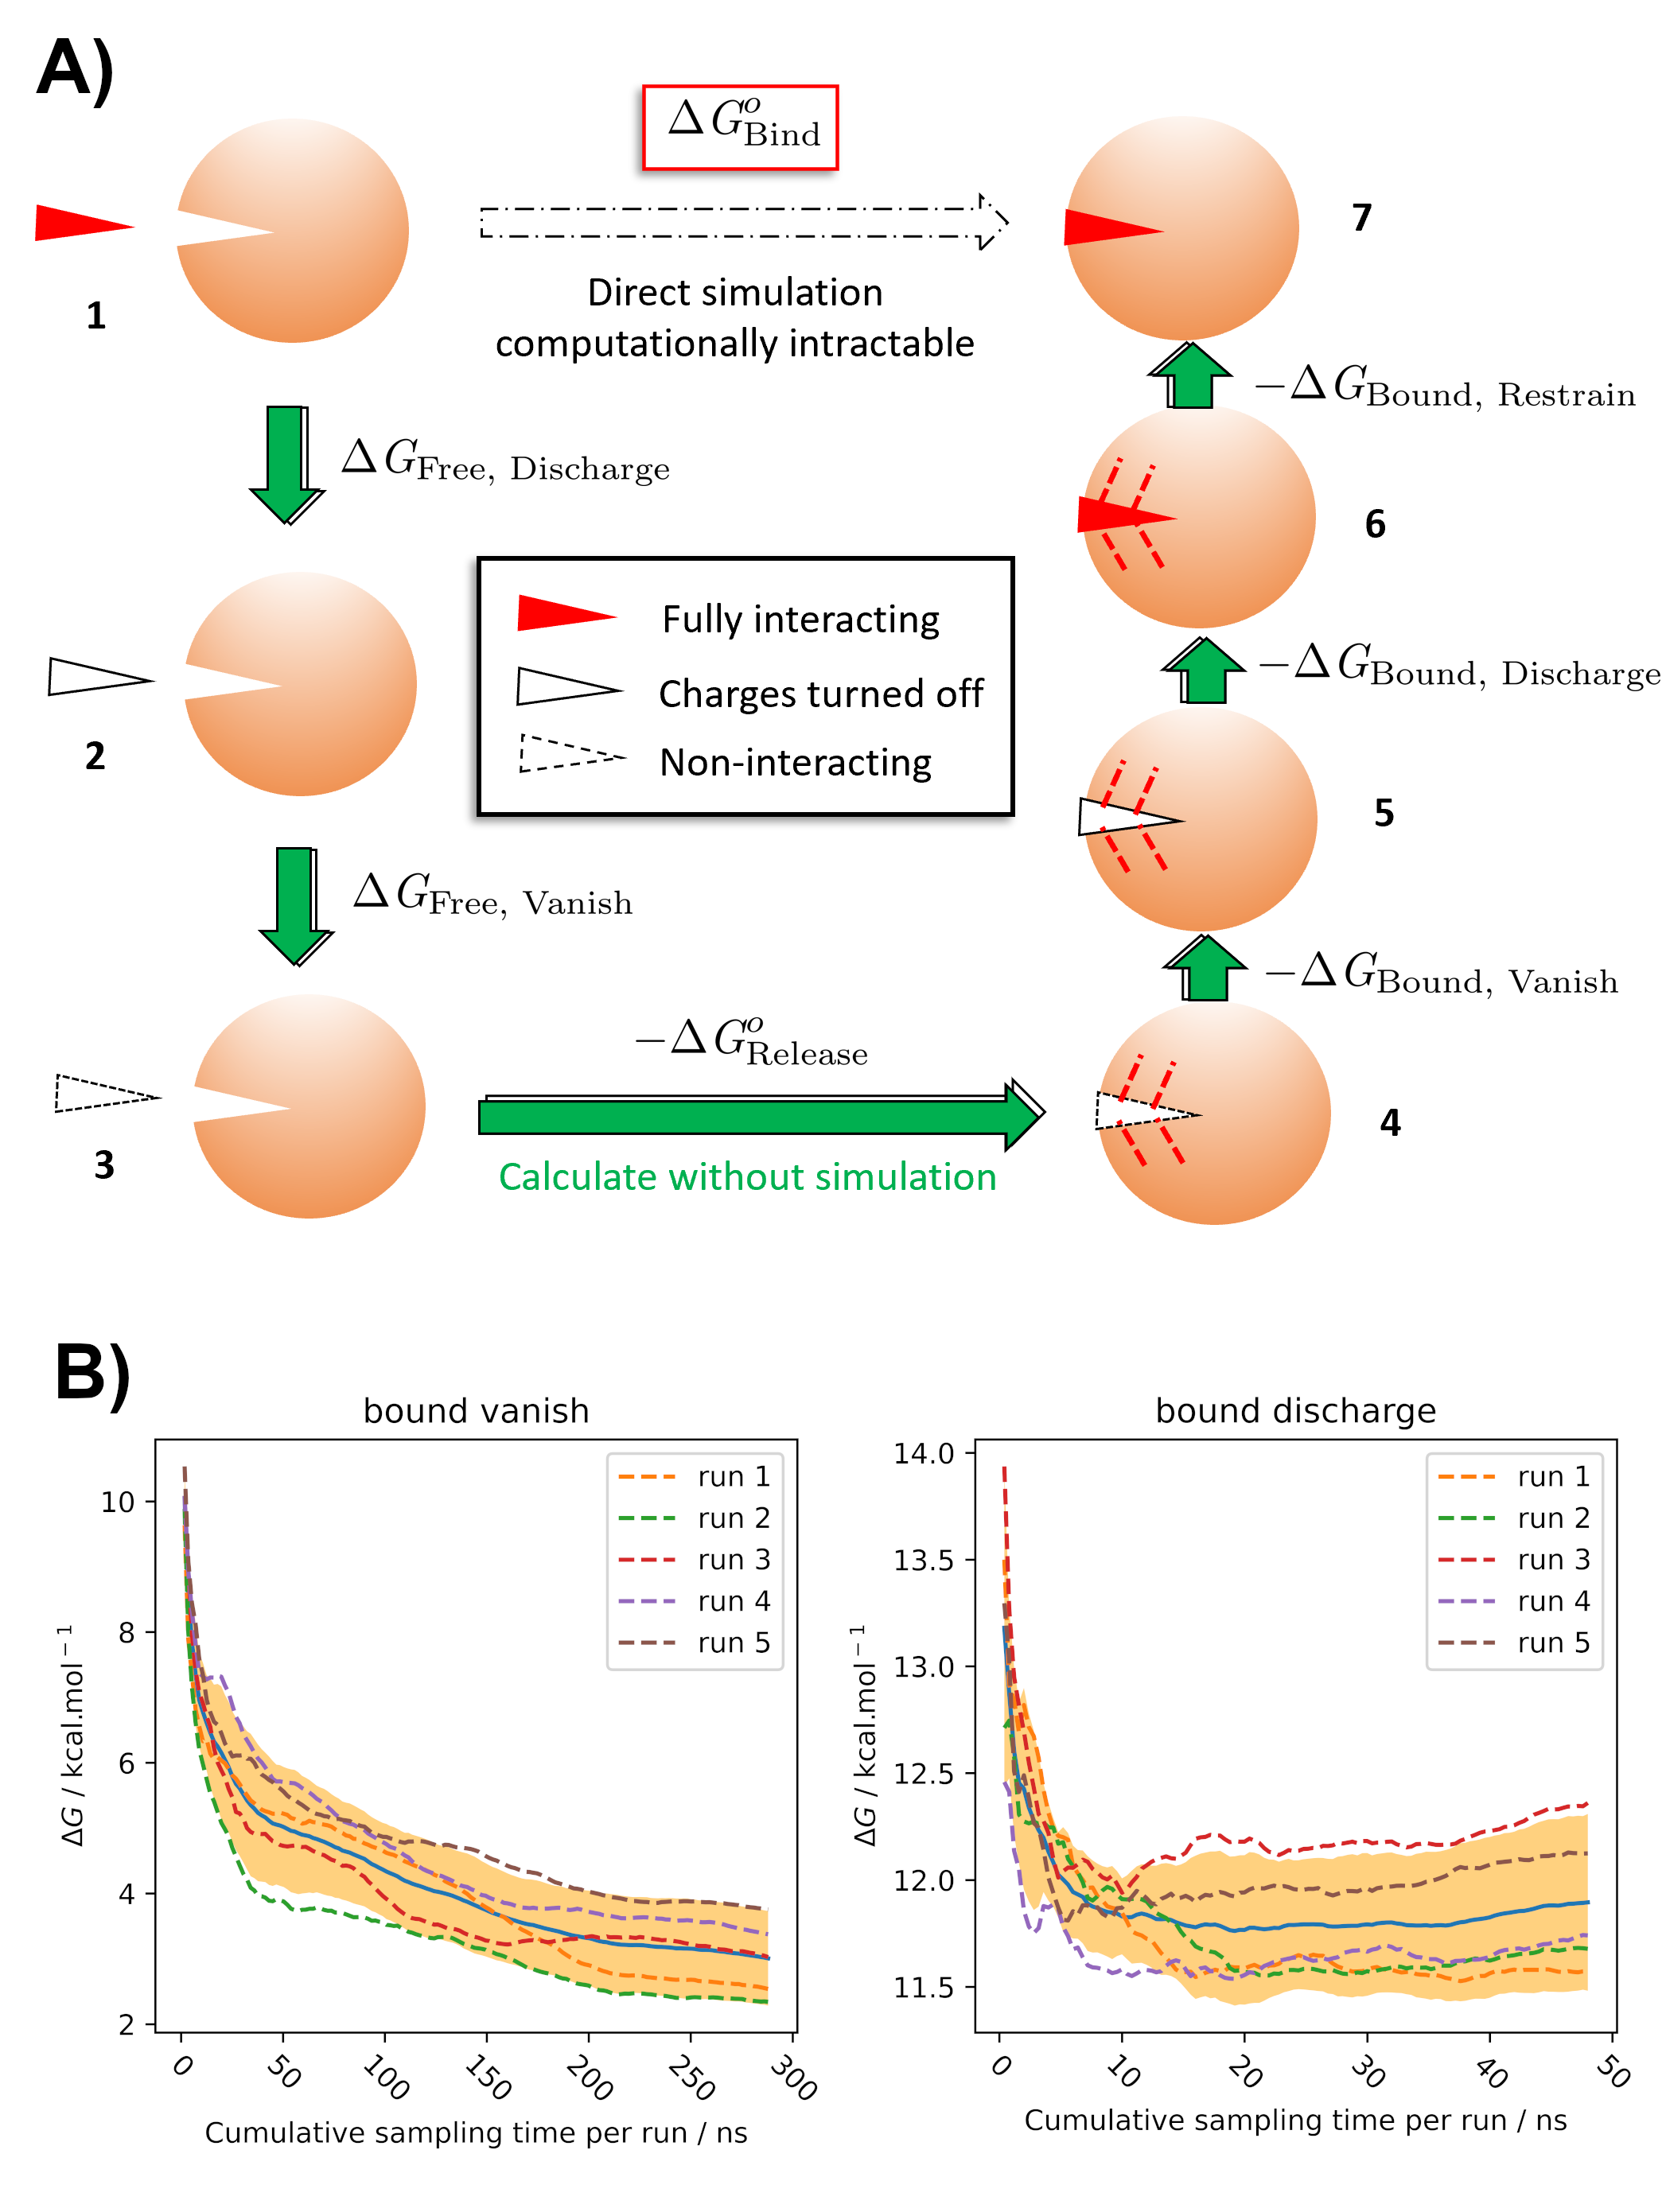
\includegraphics[width=\linewidth]{LIVECOMS/04_fep/abfe-tutorial.png}
\caption{ \textbf{A)} Thermodynamic cycle for alchemical absolute binding free energy calculations. \textbf{B)} Sample convergence plots for legs 5 and 6 of the ABFE thermodynamic cycle for the MIF/MIF180 complex, showing especially poor convergence for the bound vanish stage prior to discarding initial non-equilibrated samples.} 
\label{abfe_fig}
\end{figure}

The notebook describes the use of \textit{BSS.Align.decouple} to tag a molecule in a BSS system that should have all its intermolecular interactions removed to compute its absolute binding free energy. This is illustrated here with the use of the ligand MIF180 bound to the protein MIF \cite{Qian2019, Clark2023}. 

Next, it is shown how to run and analyse a simulation of the fully-interacting protein-ligand complex to generate the required intermolecular restraints. Both actions are handled using \textit{BSS.FreeEnergy.RestraintSearch}. The popular 6-degrees of freedom Boresch restraints are supported \cite{boresch_absolute_2003}, as well as a Clark's multiple distance restraints (MDR) methodology \cite{Clark2023}.
The notebook illustrates the automated generation of Boresch or MDR restraints with BSS. The algorithm implemented aims to select stable restraints which mimic strong native receptor-ligand interactions. The notebook includes visualization of the chosen restraints before free energy inputs are prepared, which allows the user to identify cases where the selected restraints may not be optimal, or where symmetry corrections may be required \cite{duboue-dijon_building_2021}. The notebook then demonstrates the use of \textit{BSS.FreeEnergy.AlchemicalFreeEnergy} to generate input files for the engines SOMD or GROMACS. This class in the Exscientia sandpit contains all of the functionality from \textit{BSS.FreeEnergy.Relative} in the main version of the code, as well as additional functionality required for ABFE calculations.

Since ABFE calculations can be time-consuming we recommend parallel execution of the different legs of the thermodynamic cycle using an approach similar to that used in the RBFE tutorial.
\\

The fifth notebook \href{https://github.com/OpenBioSim/biosimspace_tutorials/blob/main/04_fep/03_ABFE/02_analysis_abfe.ipynb}{02-analysis-abfe} describes how to analyse an ABFE calculation to estimate the free energy of binding of a ligand. Sample output simulation data are provided for each leg of the double decoupling thermodynamic cycle and analysed using \textit{BSS.FreeEnergy.AlchemicalFreeEnergy.Analyse} to plot potentials of mean forces. The standard free energy of binding is then obtained by summing the free energy changes from each leg and adding a standard state correction term for the use of Boresch restraints, along with any symmetry corrections required. The notebook also describes how to carry out convergence analyses (see Figure \ref{abfe_fig}B) to assess the robustness of the ABFE estimates.  


%\section{Checklists}
%Tutorials do not necessarily require the use of a checklist as in Best Practices documents; however, they can include these if desired.
%Several useful checklist formats are available, with examples presented in \texttt{sample-document.tex} in \url{github.com/livecomsjournal/article_templates/templates}.
%One example is shown here.
%
% Here is a single-column checklist that consists of multiple sub-checklists
%\begin{Checklists}
%
%\begin{checklist}{A list}
%\textbf{Single-column checklists are also straightforward by removing the asterisk}
%\begin{itemize}
%\item First thing let's do an item which breaks across lines to see how that looks
%\item Also remember
%\item And finally
%\end{itemize}
%\end{checklist}

%\begin{checklist}{Another list}
%\textbf{This is some further description.}
%\begin{itemize}
%\item First thing
%\item Also remember
%\item And finally
%\end{itemize}
%\end{checklist}
%
%\end{Checklists}

\section{Author Contributions}
%%%%%%%%%%%%%%%%
% This section mustt describe the actual contributions of
% author. Since this is an electronic-only journal, there is
% no length limit when you describe the authors' contributions,
% so we recommend describing what they actually did rather than
% simply categorizing them in a small number of
% predefined roles as might be done in other journals.
%
% See the policies ``Policies on Authorship'' section of https://livecoms.github.io
% for more information on deciding on authorship and author order.
%%%%%%%%%%%%%%%%
LH prepared Tutorial 1, DL and LH prepared Tutorial 2, AH and LH prepared Tutorial 3, JS, AK, LH, AH, FC, and JM prepared Tutorial 4, which was built on older tutorial material by AM and SB and on contributions from ZW, MS, and BC. MB and CW reviewed and tested all tutorials and ported the tutorials to a web server. The authors are listed in alphabetical order, with the exception of the first coauthor.
% We suggest you preserve this comment:
For a more detailed description of author's contributions,
see the GitHub issue tracking and changelog at \githubrepository.

\section{Other Contributions}
%%%%%%%%%%%%%%%
% You should include all people who have filed issues that were
% accepted into the paper, or that upon discussion altered what was in the paper.
% Multiple significant contributions might mean that the contributor
% should be moved to authorship at the discretion of the a
%
% See the policies ``Policies on Authorship'' section of https://livecoms.github.io for
% more information on deciding on authorship and author order.
%%%%%%%%%%%%%%%
Gratitude is expressed to the users of BioSimSpace who have given important feedback over the past years that have influenced the production of our tutorials and documentation. 
% We suggest you preserve this comment:
For a more detailed description of contributions from the community and others, see the GitHub issue tracking and changelog at \githubrepository.

\section{Potentially Conflicting Interests}
%%%%%%%
%Declare any potentially competing interests, financial or otherwise
%%%%%%%
JM is a member of the Scientific Advisory Board of Cresset. 

\section{Funding Information}
%%%%%%%
% Authors should acknowledge funding sources here. Reference specific grants.
%%%%%%%
JM acknowledges support from an EPSRC standard grant (EP/P022138/1) and from the University of Edinburgh UCB via an EPSRC-Impact Acceleration Account (IAA PIII074).

\section*{Author Information}
\makeorcid

\bibliography{references}

%%%%%%%%%%%%%%%%%%%%%%%%%%%%%%%%%%%%%%%%%%%%%%%%%%%%%%%%%%%%
%%% APPENDICES
%%%%%%%%%%%%%%%%%%%%%%%%%%%%%%%%%%%%%%%%%%%%%%%%%%%%%%%%%%%%

%\appendix


\end{document}